\documentclass{moncours}
\usepackage{minted}
\usepackage{float}
%\usepackage{pygmentize}




\makeindex




\begin{document}

\newcounter{tmp} % pour couper les boîtes énoncés au milieu d'un enumerate

\renewcommand{\labelitemi}{\textbullet}
\renewcommand{\labelitemii}{$\circ$} 

\frontmatter

\titlePage[./images/couvertureFlo3e_v1]{Informatique 3\up{e}}{Fiches MITIC}{Institut Florimont}{Petit-Lancy (Suisse)\\ \textcopyright\ Tout droit réservé. Crédit photographie couverture : Institut Florimont. Illustration des premières pages de chapitre issue de \emph{Codex Leicester} de Leonardo da Vinci (domaine public). \\1\up{ère} édition, v1.0 \\ juin 2021} 

% TOC
\pagestyle{empty} % No headers

\tableofcontents % Print the table of contents itself
\cleardoublepage % Forces the first chapter to start on an odd page so it's on the right
\pagestyle{fancy} % Print headers again

%\cleardoublepage % on force une page impaire
%\vspace*{1cm}

\section*{Calendrier des différentes activités (5\up{e})}\index{Calendrier des activités}  

\vfill

\begingroup % permet de bloquer le arraystretch à ce groupe seulement
\renewcommand{\arraystretch}{1.2}
\begin{center}
\begin{tabular}{|l|l|c|l|l|}
\hline
\multirow{2}{*}{\textbf{Nom de la fiche}} & \multirow{2}{*}{\textbf{Matière}} & \multirow{2}{*}{\textbf{Page}} & \textbf{Date de} & \textbf{Nom du} \\
 &  &  & \textbf{réalisation} & \textbf{professeur} \\ \hline
%\rowcolor[gray]{0.8}\multicolumn{5}{|l|}{Rentrée scolaire} \\ \hline 
%\emph{La plateforme Flore} & (Titulaire) & \pageref{plateformeFlore} & & \phantom{xxxxxxxxxxxxxxxx}  \\ \hline
%
% avant les vacances d'octobre
%
\rowcolor[gray]{0.8}\multicolumn{5}{|l|}{Avant les vacances d'octobre} \\ \hline
\emph{Tableur : séance 1} & Physique-Chimie & \pageref{ficheTableur5e1} & & \\ \hline
\emph{Texte : séance 1} & Français & \pageref{ficheTexte5e1} & & \\ \hline \hline
%
% avant les vacances de Noël
%
\rowcolor[gray]{0.8}\multicolumn{5}{|l|}{Avant les vacances de Noël} \\ \hline
\emph{Tableur : séance 2} & Mathématiques & \pageref{ficheTableur5e2} & & \\ \hline

\emph{Scratch : séance 1} & Mathématiques & \pageref{ficheScratch5e1} & & \\ \hline \hline
%
% avant les vacances de février
%
%\rowcolor[gray]{0.8}\multicolumn{5}{|l|}{Avant les vacances de février} \\ \hline
%
% avant les vacances de printemps
%
\rowcolor[gray]{0.8}\multicolumn{5}{|l|}{Avant les vacances de printemps} \\ \hline
\emph{Texte : séance 2} & Anglais & \pageref{ficheTexte5e2} & & \\ \hline
\emph{Scratch : séance 2} & Mathématiques & \pageref{ficheScratch5e2} & & \\ \hline
\emph{Son : séance 1} & Anglais & \pageref{ficheSon5e1} & & \\ \hline \hline
%
% avant les vacances d'été
%
\rowcolor[gray]{0.8}\multicolumn{5}{|l|}{Avant les vacances d'été} \\ \hline
\emph{Image : séance 1} & Français & \pageref{ficheImage5e1} & & \\ \hline
\emph{Scratch : séance 3} & Mathématiques & \pageref{ficheScratch5e3} & & \\ \hline \hline
%
% avant la fin du semestre de cours
%
\rowcolor[gray]{0.8}\multicolumn{5}{|l|}{Avant la fin du semestre de cours (pour les cours au semestre)} \\ \hline
\emph{Tableur : séance 3} & Géographie & \pageref{ficheTableur5e3} & & \\ \hline
\emph{Texte : séance 3} & Histoire & \pageref{ficheTexte5e3} & & \\ \hline
\emph{Image : séance 2} & Arts visuels & \pageref{ficheImage5e2} & & \\ \hline
%\emph{Son : séance 2} & Musique & \pageref{ficheSon5e2} & & \\ \hline
\end{tabular}
\end{center}
\endgroup

\vfill

\cleardoublepage % on force une page impaire pour le clavier
\section*{Les touches spéciales du clavier}\index{Clavier}\index{Touches spéciales}

\vfill

\begin{center}
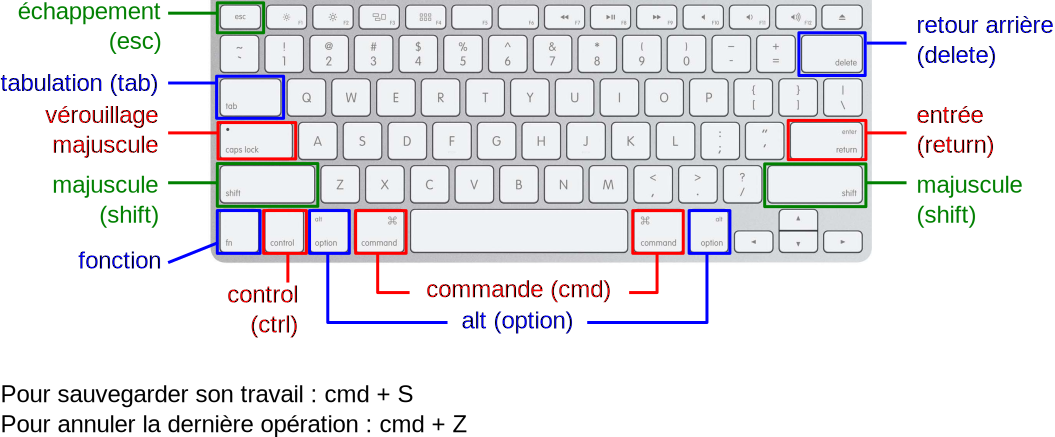
\includegraphics[angle=90,width=.6\textwidth]{./images/generales/clavierTouches}
\end{center}

\vfill

%\cleardoublepage % on force une page impaire pour la philosophie du document
%\chapter*{Philosophie du document}


\prof{\textbf{ceci est la version professeur du document.} L'icône du professeur est suivie par des informations complémentaires qui n'apparaissent pas dans la version élève.}  

Vous avez entre les mains le deuxième tome d'une série de trois fascicules qui accompagneront les élèves des classes de 6\up{e}, 5\up{e} et 4\up{e} jusqu'au moment où ils recevront un ordinateur qu'ils seront en mesure d'exploiter au mieux pour leur travail.

\vspace{18pt}

Ce document se présente sous la forme d'un livret qui rassemble des fiches MITIC\footnote{MITIC : Médias, Images et Technologies de l'Information et de la Communication.} permettant aux élèves d'apprendre à utiliser les logiciels et espaces numériques mis à leur disposition. Pour l'année de 5\up{e}, sont traités les logiciels \emph{Microsoft Word} (traitement de texte), \emph{Microsoft Excel} (tableur grapheur), \emph{Gimp} (retouche d'image), \emph{Audacity} (traitement des fichiers son) et \emph{Scratch} (programmation). Au début de chaque chapitre un lien permettant de télécharger le logiciel est fourni.

\vspace{18pt}


Chaque fiche est conçue pour être exploitée à plusieurs occasions et dans des matières différentes, à chaque fois lors d'une séance de 45 minutes. La fiche sur le tableur, par exemple, est découverte en physique-chimie (\emph{Séance 1}), exploitée à nouveau en mathématiques (\emph{Séance 2}) puis en histoire-géographie (\emph{Séance 3}) selon un calendrier proposé en début de fiche. Nous avons à chaque fois essayé de faire coïncider les notions abordées dans la fiche avec le programme de la matière concernée.

\vspace{18pt}
\prof{
Professeurs, c'est à vous que revient la tâche délicate d'inclure le contenu de ces fiches dans votre progression. À vous de le faire vivre : arriver en salle informatique et demander aux élèves de remettre en forme un texte de Molière ne présente que peu d'intérêt pédagogique. Donnez du sens à ces fiches et profitez-en pour diversifier votre enseignement. N'hésitez pas à exploiter dans vos cours les techniques présentées dans ce fascicule afin que les élèves utilisent plusieurs fois leurs nouvelles compétences et, par là-même, les pérennisent.
}
%\vspace{18pt}

%Ces fiches MITIC sont appelées à évoluer. N'hésitez pas à nous transmettre vos suggestions et nous signaler toute erreur relevée par courriel à l'adresse \texttt{flo-mitic@florimont.ch}.

%\vspace{18pt}

Merci d'avance à tous pour votre implication.

\vspace{18pt}

L'équipe de rédaction.

\vspace{2cm}

% \emph{Remarque : il existe une version professeur de ce document, contenant des informations complémentaires, disponible sur l'ENT de l'école.}

  


% Début des chapitres
\setcounter{page}{1} % si on veut forcer la page 1 au début du premier chapitre
\mainmatter
%
  
\begin{minted}{python}
import sympy as sy
\end{minted}

\chapterImage{./images/chapitreVinci4e.png}
%\input{./sources/activite1/activite1.tex}
\chapter{Découverte Python et module Turtle}\index{decouvertePython}

Python est un langage de programmation très implanté dans les milieux éducatif et scientifique de par la clarté de sa grammaire et l'efficacité de son code. Nous allons apprendre dans cette activité à faire le lien entre la programmation Scratch telle que vous l'avez vue en classes de 6\up{ème}, 5\up{ème}, 4\up{ème} et la programmation Python. Cette initiation en douceur à Python va donc vous permettre de découvrir les bases de ce langage. 

\section{Pour bien commencer}

Vous devrez utiliser \emph{Pyzo} pour exécuter votre code Python. \emph{Pyzo} est un éditeur de programme léger permettant d'exécuter du code Python. 

Ouvrir l'éditeur \emph{Pyzo} en cliquant d'abord sur l'icône 
\includegraphics[width=1cm]{./images/activite7/icone_recherche} puis en complétant la barre de recherche : 

\uneimageici{./images/activite7/recherche_pyzo.png}{.5\textwidth} % reprise image existante

\emph{Pyzo} s'ouvre et vous propose deux zones distinctes de travail :
\begin{itemize}
\item à gauche l'éditeur dans lequel vous allez taper votre code,
\item à droite la console dans laquelle vont apparaître les erreurs de code et les résultats fournis après avoir exécuté le code Python.
\end{itemize}

\uneimageici{./images/activite7/ecran_pyzo.png}{.8\textwidth}% reprise image existante

Commencez par créer un nouveau fichier. Pour cela, sélectionner \texttt{Nouveau} dans le menu \texttt{Fichier}

\uneimageici{./images/activite7/nouveau_fichier.png}{.4\textwidth} % reprise image existante

Puis enregistrez votre fichier au format \texttt{Nom-date.py}

\section{L'activité demandée}



\subsection{Partie Scratch}

En utilisant le logiciel \emph{Scratch}, écrire un script qui dessine un carré.

\uneimageici{./images/activite2/scratch_uncarre.png}{.1\textwidth}

Ecrire ensuite un autre script permettant d'obtenir une suite de trois carrés. 

\uneimageici{./images/activite2/scratch_troiscarres.png}{.3\textwidth}

Par exemple, le code suivant vous permet d'obtenir le résultat escompté

\uneimageici{./images/activite2/codescratch_troiscarres.png}{.2\textwidth}

\subsection{Partie Python}

Nous allons maintenant traduire bloc par bloc en Python le code obtenu dans la première partie.\\

Le bloc suivant

\uneimageici{./images/activite2/scratch_demarrerScript.png}{.15\textwidth}

correspond à l'exécution du code Python sur \emph{Pyzo}

\uneimageici{./images/activite7/executer_fichier.png}{.4\textwidth} % image deja existante

\begin{minted}{python}
from turtle import *
def carre():
color("red")
begin_fill()
for i in range(4}:
down()
forward(50)
left(90)
end_fill()

def ligne():
for i in range(3):
carre()
up()
forward(60)

x = 0
y = 0
for i in range(3):
goto(x, y)
ligne()
x = 0
y = y - 60
\end{minted}
%\newpage

\section{Tracer des courbes et surfaces en Python}\index{courbesPython}

\subsection{Pour bien commencer}

Vous devrez utiliser \emph{Pyzo} pour exécuter votre code Python. \emph{Pyzo} est un éditeur de programme léger permettant d'exécuter du code Python. 

Ouvrir l'éditeur \emph{Pyzo} en cliquant d'abord sur l'icône 
\includegraphics[width=1cm]{./images/activite7/icone_recherche} puis en complétant la barre de recherche : 

\uneimageici{./images/activite7/recherche_pyzo.png}{.5\textwidth} % reprise image existante

\emph{Pyzo} s'ouvre et vous propose deux zones distinctes de travail :
\begin{itemize}
\item à gauche l'éditeur dans lequel vous allez taper votre code,
\item à droite la console dans laquelle vont apparaître les erreurs de code et les résultats fournis après avoir exécuté le code Python.
\end{itemize}

\uneimageici{./images/activite7/ecran_pyzo.png}{.8\textwidth}% reprise image existante

Commencez par créer un nouveau fichier. Pour cela, sélectionner \texttt{Nouveau} dans le menu \texttt{Fichier}

\uneimageici{./images/activite7/nouveau_fichier.png}{.4\textwidth} % reprise image existante

Puis enregistrez votre fichier au format \texttt{Nom-date.py}



%
%
%  S  É  A  N  C  E     S  U  R     L  E  S     R  A  Y  O  N  S      A  T  O  M  I  Q  U  E  S
%
%

\chapter{Séance 4 : Rayon atomique}\label{ficheTableur4e1}

Le but de cette séance est d'utiliser python pour afficher un graphique montrant le rayon atomique en fonction du numéro de l'atome correspondant.

\section{Pour bien démarrer...}

Pour commencer, ouvrez \emph{Excel} et créez un fichier que vous allez nommer \texttt{Elements.csv} (Sauvegardez-le tout de suite pour être sûrs de ne pas le perdre par la suite.) Ce fichier contiendra les données que nous allons ensuite afficher sur le graphique. Pendant que vous travaillez, pensez à sauvegarder régulièrement votre travail (raccourci clavier \texttt{Cmd + s}).   

\uneimageici{./images/generales/clavierCmdS}{.4\textwidth}


\section{L'activité demandée}

\boiteEnonceLarge{%

%\vspace{6pt}

Pour compléter le fichier \texttt{Elements.csv}, il faut:

\begin{itemize}
\item Créer les en-têtes du document, nommées \texttt{numéro atomique} et \texttt{rayon atomique (pm)};
\item Remplir la colonne du numéro atomique par les nombres entiers de 1 à 20;
\item Remplir la colonne du rayon atomique par la valeur du rayon atomique associée aux vingt premiers éléments. Pour trouver ces valeurs, une recherche sur internet peut être requise. Assurez-vous que les valeurs soient bien exprimées en picomètres (pm) ou convertissez-les si ce n'est pas le cas.
\end{itemize}
%\vspace{10pt}
} % fin 

\vfill
\phantom{rien}

\boiteEnonceLarge{%
Une fois cela fait, enregistrez le fichier à nouveau. Il va maintenant falloir l'ouvrir grâce à un code python. Vous disposez d'un tel code (mis à votre disposition par votre enseignant) nommé \texttt{$graphique\_rayon\_atomique.py$}. Vérifiez qu'il se trouve bien dans le même dossier que votre fichier \texttt{Elements.csv}.
Lancez le code, il devrait ouvrir une fenêtre avec un graphique tel que présenté ci-dessous.

\uneimageici{./images/activite4/graphique_pre_modif.png}{.6\textwidth}

Certains éléments de ce graphique sont à revoir, vous allez les modifier.

\begin{itemize}
\item Pour commencer, ajoutez l'unité (pm) à l'axe des ordonnées;
\item Ajoutez un titre approprié au graphique en ajoutant une ligne \texttt{plt.title('Titre du graphique')} et en y remplaçant "Titre du graphique" par ce que vous voulez;
\item Modifiez la courbe en remplaçant la couleur par du bleu.
\end{itemize}
\vspace{10pt}
Une fois ces modifications terminées, enregistrez votre code et exécutez-le à nouveau : vous devriez apercevoir une versions à jour du graphique. Si vous essayez de modifier les valeurs du document .csv, vous obtiendrez alors une courbe différente.\\

Maintenant que votre travail est terminé, enregistrez le graphique au format PNG (le fichier doit être nommé à partir de votre nom : \texttt{Nom-seance4.png}), puis vous le rendrez sur \emph{Teams} à l'endroit indiqué par votre enseignant (si nécessaire, se reporter à la fiche méthode \emph{Remettre son devoir}, page \pageref{TeamsRemettreDevoir}).
} % fin 

\section{Pour aller plus loin...}
Vous avez modifié un code Python pour personnaliser un graphique, mais on peut faire beaucoup plus!
\begin{itemize}
\item Si vous ajoutez quelques lignes de plus à votre document .csv, que va-t-il se passer?
\item On peut ajouter des colonnes au fichier .csv avec d'autres informations concernant les éléments (masse atomique, électronégativité, etc...) et faire des graphiques similaires, ou même les comparer entre elles. Essayez par exemple de faire un graphique représentant la masse des éléments en fonction de leur numéro atomique;
\item On peut créer plusieurs courbes sur le même graphique pour voir s'il y a des corrélations entre certaines valeurs. Par exemple, vous pouvez tracer la courbe de l'électronégativité en fonction du numéro atomique en plus de celle du rayon atomique et voir s'il y a un point commun entre ces courbes ou non;
\item Modifier l'aspect de la courbe en ajoutant par exemple {plt.rcParams['lines.linestyle'] = '--'}. Cette ligne peut être modifiée pour afficher la courbe sous d'autres formes;
\item Ajouter un affichage des points en plus de la courbe pour une lecture plus claire des résultats..
\end{itemize}

\vfill

%\cadre{Pensez à sauver régulièrement votre travail en appuyant sur \texttt{Cmd + S} ou à partir du menu \texttt{Fichier} en choisissant \texttt{Enregistrer}.

%\uneimageici{./images/generales/clavierCmdS}{.5\textwidth}
%}


%\input{./sources/activite5/activite5.tex}
%\input{./sources/activite6/activite6.tex}
\newpage

\section{Factorisation et développement}\index{factorisationDeveloppement}

Vous avez appris à factoriser et développer des expressions mathématiques. C'est parfois difficile mais cela vous permet de résoudre certains problèmes dont vous ne pourriez trouver la solution autrement. Le langage Python permet d'obtenir un résultat similaire à moindre effort si on sait l'utiliser correctement. Savoir utiliser cet outil pour trouver vos résultats ou vérifier votre travail est une donc compétence bien utile que vous allez apprendre aujourd'hui.\\

\subsection{Pour bien commencer...}

Vous devrez utiliser \emph{Pyzo} pour exécuter votre code Python. \emph{Pyzo} est un éditeur de programme léger permettant d'exécuter du code Python. 

Ouvrir l'éditeur \emph{Pyzo} en cliquant d'abord sur l'icône 
\includegraphics[width=1cm]{./images/activite7/icone_recherche} puis en complétant la barre de recherche : 

\uneimageici{./images/activite7/recherche_pyzo.png}{.5\textwidth}

\emph{Pyzo} s'ouvre et vous propose deux zones distinctes de travail :
\begin{itemize}
\item à gauche l'éditeur dans lequel vous allez taper votre code,
\item à droite la console dans laquelle vont apparaître les erreurs de code et les résultats fournis après avoir exécuté le code Python.
\end{itemize}

\uneimageici{./images/activite7/ecran_pyzo.png}{.8\textwidth}

Commencez par créer un nouveau fichier. Pour cela, sélectionner \texttt{Nouveau} dans le menu \texttt{Fichier}

\uneimageici{./images/activite7/nouveau_fichier.png}{.4\textwidth}

Puis enregistrez votre fichier au format \texttt{Nom-date.py}


\subsection{L'activité demandée}

\vspace{12pt}

\subsubsection{Etape 1 - calcul manuel}

\vspace{12pt}

\boiteEnonceLarge{% début énoncé étape 1
Dans un premier temps, soyez courageux et effectuez les calculs suivants à la main, afin de comparer plus tard vos résultats et ceux de l'ordinateur.\\

\emph{Exercice 1}\\

Factoriser l'epression suivante : $A=(x-1)(2x+7)+3(1-x)(5-x)$\\

\emph{Exercice 2}\\

Développer l'expression suivante : $B=5(2x-7)(3-x+x^2)$\\

\emph{Exercice 3}\\

Simplifier l'expression suivante : $C=\frac{144x^2+84}{8}$\\

\emph{Exercice 4}\\

Résoudre l'équation suivante : $D=(9-x^2)(3x-1)=4(x-3)(2x+5)$
}% fin énoncé étape 1

\subsubsection{Etape 2 - Python}

\vspace{12pt}

Pour exécuter les codes ci-dessous, vous pouvez sélectionner \texttt{Démarrer le script} dans le menu  \texttt{Exécuter}

\uneimageici{./images/activite7/executer_fichier.png}{.4\textwidth}

\vfill
\phantom{rien}

\boiteEnonceLarge{% début énoncé
Nous allons maintenant retrouver les résultats précédents en utilisant des codes simples du langage Python.\\

En Python, le calcul littéral nécessite l'importation d'un module appelé \emph{sympy}, puis l'affectation de symboles formels \emph{x, y, z, ...} aux différentes variables \texttt{x, y, z, ...} Pour cela, commencez votre code par\\

\texttt{from sympy import *}\\
\texttt{x, y, z = symbols('x y z')}\\

\emph{Exercice 1}\\

Pour factoriser une expression \texttt{E}, \emph{sympy} utilise \texttt{factor(E)}.\\

Par exemple, on sait que $(x-1)(x+2)+(x-1)(x+3)=(x-1)(2x+5)$. Essayez donc dans votre fenêtre \emph{Pyzo} l'instruction Python \\

\texttt{print(factor((x-1)*(x+2)+(x-1)*(x+3)))} \\

pour retrouver ce résultat. \\

Vous remarquerez qu'en Python, les produits s'expriment avec \texttt{*} \\

Essayez maintenant d'obtenir à l'aide de Python le résultat que vous aviez trouvé manuellement pour l'exercice 1.\\

\emph{Exercice 2}\\

Pour développer une expression \texttt{E}, \emph{sympy} utilise \texttt{expand(E)}.\\

Par exemple, on sait que $(x-1)(x-2)=x^2-3x+2$. Essayez donc dans votre fenêtre \emph{Pyzo} l'instruction Python \\

\texttt{print(expand((x-1)*(x-2)))}  \\

pour retrouver ce résultat.\\

Essayez maintenant d'obtenir à l'aide de Python le résultat que vous aviez trouvé manuellement pour l'exercice 2.
}%fin énoncé

\boiteEnonceLarge{% debut enonce
\emph{Exercice 3}\\

Pour simplifier une expression \texttt{E}, \emph{sympy} utilise \texttt{simplify(E)}.\\

Par exemple, on sait que pour $x\ne0$, on peut écrire $\frac{2x^2+6x}{2x}=x+3$. Essayez donc dans votre fenêtre \emph{Pyzo} l'instruction Python \\

\texttt{print(simplify(2*x**2+6*x)/(2*x))}  \\

pour retrouver ce résultat. \\

Vous remarquez qu'en Python, les puissances peuvent s'exprimer avec \texttt{**} \\ 

Essayez maintenant d'obtenir à l'aide de Python le résultat que vous aviez trouvé manuellement pour l'exercice 3.\\

\emph{Exercice 4}\\

Pour résoudre une équation  \texttt{E}, \emph{sympy} utilise \texttt{solve(E, x)}.\\

Par exemple, on sait que la solution de l'équation $3x+2=0$ est $-\frac{2}{3}$. Essayez donc dans votre fenêtre \emph{Pyzo} l'instruction Python \\

\texttt{print(solve(3*x+2, x))}  \\

pour retrouver ce résultat.\\

Essayez maintenant d'obtenir à l'aide de Python le résultat que vous saviez trouvé manuellement pour l'exercice 4.\\

Une fois les vérifications terminées, vous enregistrerez votre fichier au format PY (le fichier doit être nommé à partir de votre nom : \texttt{Nom-date.py}), puis vous le rendrez sur \emph{Teams} à l'endroit indiqué par votre enseignant (si nécessaire, se reporter à la fiche méthode \emph{Remettre son devoir}, page \pageref{TeamsRemettreDevoir}).
} % fin énoncé

\subsection{Pour aller plus loin...}

On peut également factoriser et développer des expressions mathématiques, dans le module \emph{Calcul littéral} du logiciel \emph{Geogebra}. Cette méthode ne nécessite pas l'utilisation de code car \emph{Geogebra} s'exécute en utilisant une interface graphique, et bien qu'elle s'avère plus intuitive, elle est aussi plus limitée dans son utilisation.








%\input{./sources/activite8/activite8.tex}
%\input{./sources/activite9/activite9.tex}
%\input{./sources/activite10/activite10.tex}
%\input{./sources/activite11/activite11.tex}
\chapter{Annexe - Microsoft Teams}\label{teams1}  


La suite Microsoft comporte plusieurs applications qui possèdent des fonctionnalités différentes. En particulier, on notera les applications suivantes :\\

\begin{itemize}
\item \textit{Word} - est un éditeur de traitement de texte.
\item \textit{Excel} - est un tableur offrant une organisation visuelle des données et des outils d'analyse de contenu.
\item \textit{PowerPoint} - permet de créer des présentations.
\item \textit{Outlook} - est un outil de gestion des e-mails proposant un calendrier.
\item \textit{OneNote} - est un éditeur de prises de notes.
\item \textit{OneDrive} - est un cloud permettant de stocker des données sur des serveurs distants.
\item \textit{Teams} - est un outil centralisé permettant le travail collaboratif. Il gère notamment l'accès à OneNote, OneDrive ainsi qu'à la messagerie instantanée et Ourlook.
%\item \textit{Access} - est un gestionnaire de bases de données permettant la création d'applications commerciales.
%\item \textit{Edge} - est un navigator permettant l'accès à Internet.
%\item \textit{Skype} - est un gestionnaire de communication pour les appels et le chat.
%\item \textit{Sway} - est un outil de création de rapports et de newsletters interactives.
\end{itemize} 


% CONNEXION A OFFICE
\section{Connexion à Office 365 et Teams}

Ouvrez le navigateur internet de votre choix ou Safari et entrez l'URL suivante: \url{www.office.com}. Cliquez sur \textit{Connexion}.

\begin{figure}[H]
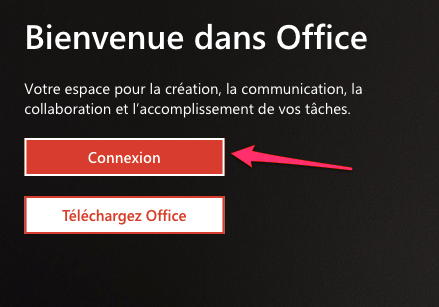
\includegraphics[width=5cm]{./images/teams/ecran_office_com_crop}
\centering
\end{figure}

Vous arrivez sur l'écran de connexion de microsoft office en ligne. Entrez votre adresse mail de l'école (qui se termine donc par \textit{@florimont.ch}).

\begin{figure}[H]
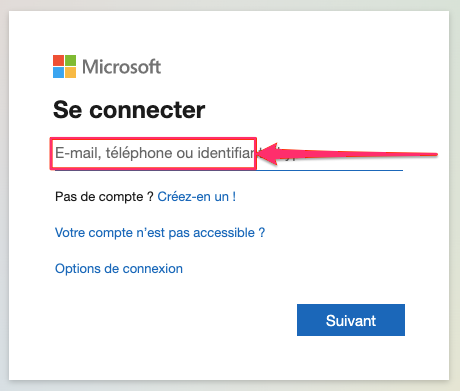
\includegraphics[width=5cm]{./images/teams/ecran_connexion_office_com_crop}
\centering
\end{figure}

Vous êtes alors redirigé vers la page d'identification de l’école. Entrez votre mot de passe. (l'adresse mail est déjà entrée, mais vous pouvez la modifier au cas où vous avez fait une erreur lors de l'étape précédente.)

\begin{figure}[H]
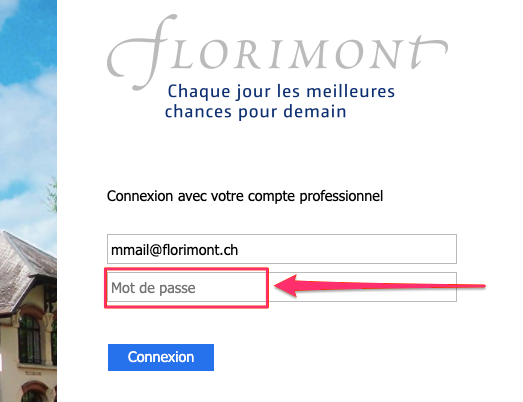
\includegraphics[width=5cm]{./images/teams/ecran_connexion_florimont_crop}
\centering
\end{figure}

Il se peut qu'on vous demande si vous voulez rester connecté. Si vous comptez travailler longtemps sur cette session, il vaut mieux accepter.\\

En revanche, si le navigateur vous propose d'enregistrer votre mot de passe, il est recommandé de refuser (soit en fermant la fenêtre, soit en choisissant \textit{Jamais}). Si vous vous connectez depuis votre ordinateur personnel, il peut être pratique de permettre au navigateur de se souvenir de mots de passe, mais ce n'est jamais une bonne idée sur un ordinateur partagé ou d'emprunt.\\

Le site vous proposera peut-être de télécharger l’application. Cliquez alors sur \textit{Utiliser l’application web à la place}.\\

Alternativement, sur certains navigateurs (comme Safari), vous devrez télécharger l'application de bureau Teams. Cliquez sur \textit{Télécharger l'application} pour continuer.

\begin{figure}[H]
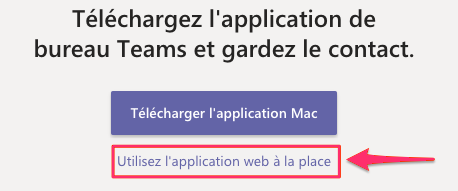
\includegraphics[width=6cm]{./images/teams/ecran_installer_teams_crop}
\centering
\end{figure}

Vous arrivez sur la page de téléchargement de l'application. Cliquez sur \textit{Download Teams}, sous le logo de la pomme, pour télécharger l'application pour Mac.\\

Vous êtes à présent dans votre espace Office. Sur la gauche, choisissez l'icône Teams.

\begin{figure}[H]
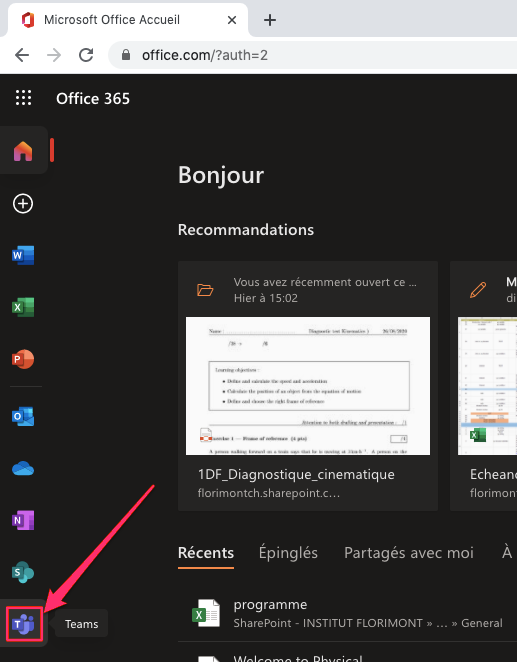
\includegraphics[width=5cm]{./images/teams/ecran_accueil_office_crop}
\centering
\end{figure}

Félicitations, vous arrivez sur la page d'accueil de votre session Teams.




% UTILISATION DE LA PUBLICATION
\section{Utilisation de la Publication}

La messagerie instantanée proposée pour chaque équipe doit permettre aux élèves et aux enseignants de communiquer en dehors de l'école dans un cadre qui reste strictement scolaire. Ainsi les messages personnels n'ont aucune raison d'être sur Teams. Il vous appartient donc de mesurer vos propos lorsque vous utilisez la messagerie instantanée. Ainsi, toute forme d'insulte ou de critique envers un membre de la classe ou une personne extérieure est à proscrire. Le modérateur de chaque équipe est son enseignant responsable.\\

Pour utiliser la messagerie, il suffit de vous rendre sur l'onglet \textit{Publications}

\begin{figure}[H]
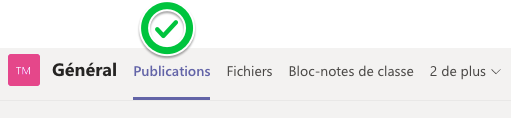
\includegraphics[width=9cm]{./images/teams/publications}
\centering
\end{figure}

puis de rédiger du texte à l'intérieur du champ \textit{Démarrer une conversation}. Utilisez @ pour mentionner un contact, ce qui signifie qu'une notification sera adressée à cette personne. Attention donc de ne pas mentionner un contact inutilement.

\begin{figure}[H]
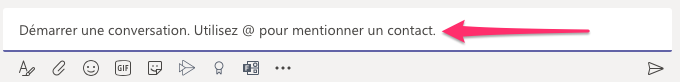
\includegraphics[width=9cm]{./images/teams/publications2}
\centering
\end{figure}

Il ne vous reste plus qu'à cliquer sur l'icône 
\includegraphics[width=0.7cm]{./images/teams/envoi_message} pour envoyer votre message.

\begin{figure}[H]
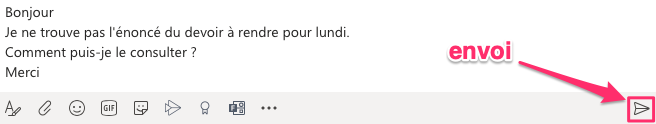
\includegraphics[width=9cm]{./images/teams/publications3}
\centering
\end{figure}





% CONSULTER ET TELECHARGER UN DOCUMENT
\section{Consulter et télécharger un document}

Vous devrez souvent chercher des documents mis en ligne par vos enseignants. Pour faire cela, sélectionnez l'onglet Fichiers, en haut.

\begin{figure}[H]
	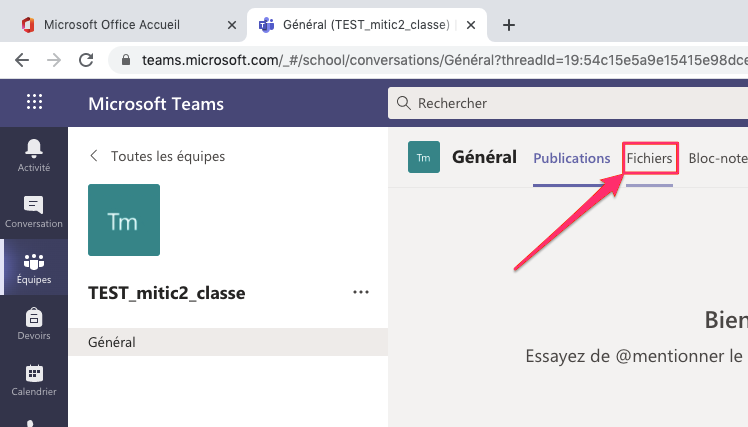
\includegraphics[width=8cm]{./images/teams/accueil_classe_crop}
	\centering
\end{figure}

Les fichiers que vos enseignants mettront à votre disposition seront la plupart du temps rangés dans un dossier. Dans cet exemple, il n'y a qu'un dossier, \textit{Support de cours}. Cliquez dessus pour l'ouvrir.

\begin{figure}[H]
	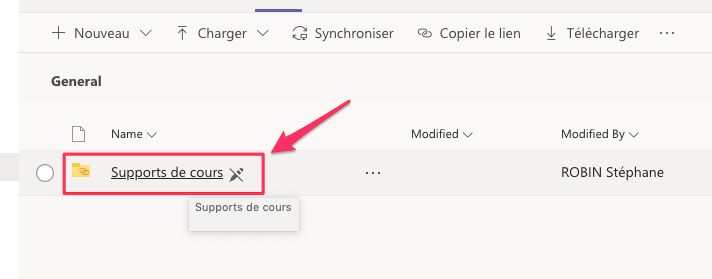
\includegraphics[width=9cm]{./images/teams/ouvrir_dossier_crop}
	\centering
\end{figure}

Vous trouverez dans ce dossier le fichier que votre professeur vous demandera de consulter. Pour le lire, il suffit de cliquer dessus.

\begin{figure}[H]
	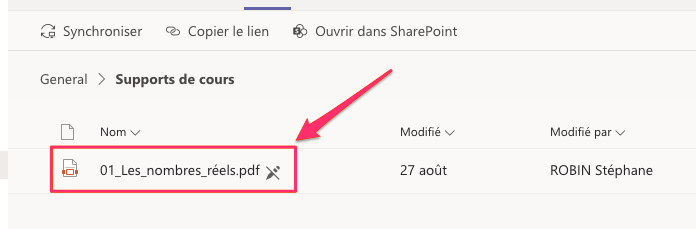
\includegraphics[width=9cm]{./images/teams/ouvrir_fichier_crop}
	\centering
\end{figure}

Vous pouvez à présent consulter le document, mais pas le modifier. Vous pouvez le télécharger pour en garder une copie sur votre ordinateur et éventuellement le modifier par la suite en cliquant sur les trois petits points en haut, puis sur \textit{Télécharger}. Une copie du document apparait alors dans votre dossier Téléchargement.\\

Une fois cela fait, vous pouvez quitter cette page pour revenir à l'affichage du dossier en cliquant sur \textit{Fermer}.
\newpage
\begin{figure}[H]
	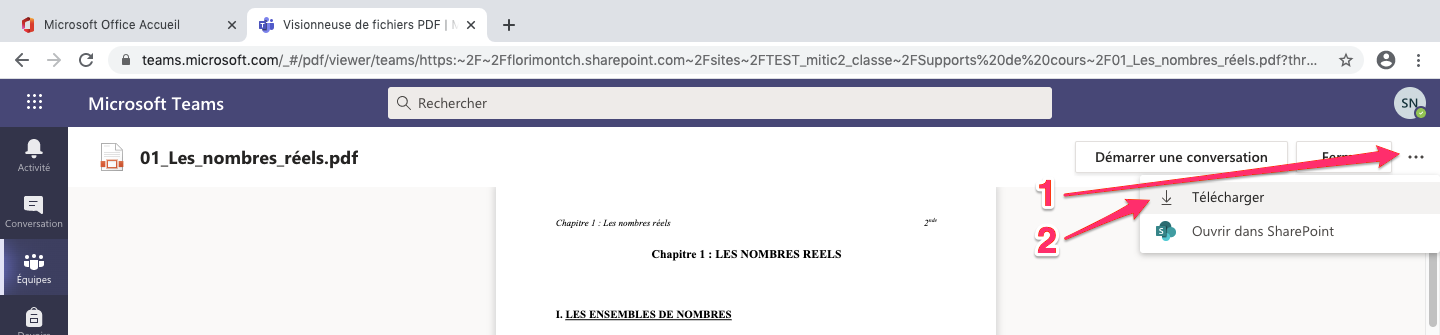
\includegraphics[width=9cm]{./images/teams/telecharger_document_crop}
	\centering
\end{figure}

Il est également possible de télécharger un document depuis la vue du dossier. Il existe plusieurs manières de faire cela. La première consiste à cliquer sur les trois petits points à côté du nom du document, puis sur \textit{Télécharger}.

\begin{figure}[H]
	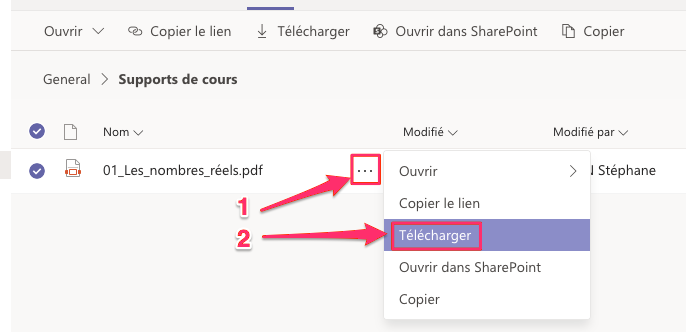
\includegraphics[width=9cm]{./images/teams/telecharger1_crop}
	\centering
\end{figure}

Alternativement, vous pouvez cliquer sur le rond à gauche du nom de fichier pour le sélectionner. Cliquez ensuite sur \textit{Télécharger}, en haut pour télécharger ce fichier. Cette dernière méthode est très pratique si vous désirez télécharger plusieurs fichiers d'un coup, car il suffit alors de les sélectionner puis de cliquer sur \textit{Télécharger} pour les récupérer en même temps.

\begin{figure}[H]
	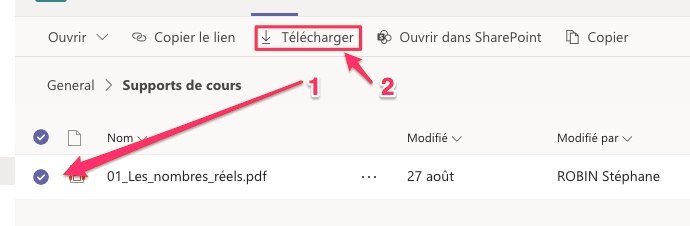
\includegraphics[width=9cm]{./images/teams/telecharger2_crop}
	\centering
\end{figure}



% DEPOSER UN DEVOIR
\section{Les devoirs}

\subsubsection{Consulter le sujet d'un devoir en pièce jointe}\label{consulterDevoir}
Pour consulter les devoirs déposés par votre enseignant, il faut choisir \textit{2 de plus} dans la barre de menus du haut de page, puis sélectionner \textit{Devoirs}.

\begin{figure}[H]
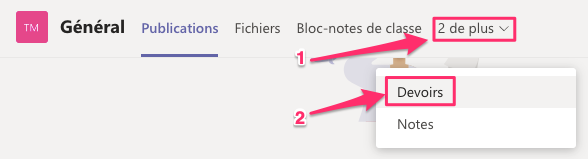
\includegraphics[width=9cm]{./images/teams/devoir1}
\centering
\end{figure}

La page qui s'affiche maintenant fait le bilan de ce qui a déjà été fait et des devoirs proposés par votre enseignant. En cliquant sur \textit{Rédaction} vous pourrez accéder au devoir.

\begin{figure}[H]
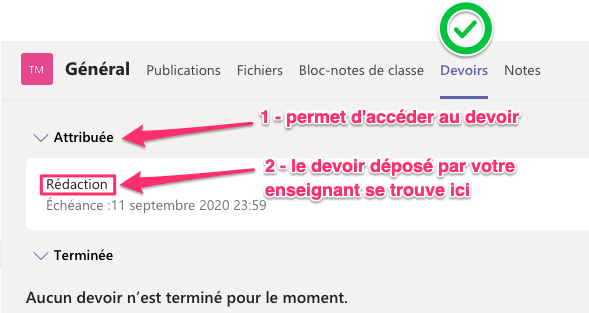
\includegraphics[width=9cm]{./images/teams/devoir2}
\centering
\end{figure}

Vous obtenez alors l'écran suivant

\begin{figure}[H]
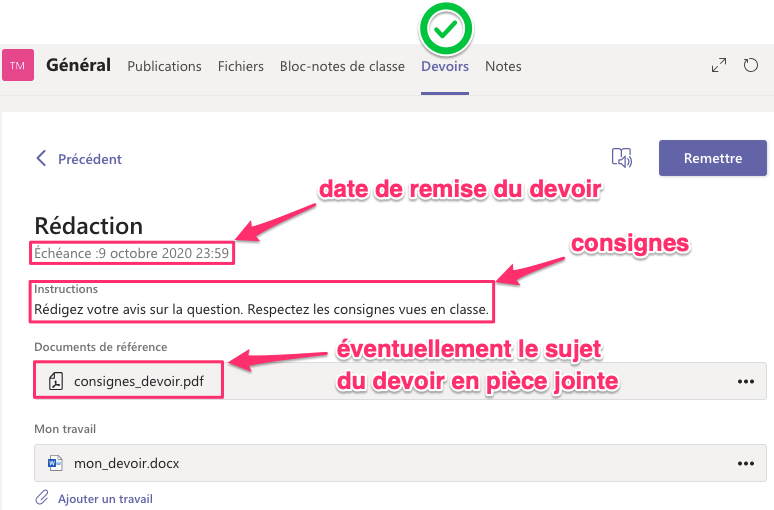
\includegraphics[width=9cm]{./images/teams/devoir3}
\centering
\end{figure}

Il est maintenant possible de consulter le sujet en sélectionnant l'icône 
\includegraphics[width=0.7cm]{./images/teams/pointilles} qui vous offre le choix entre une lecture en ligne ou un téléchargement

\begin{figure}[H]
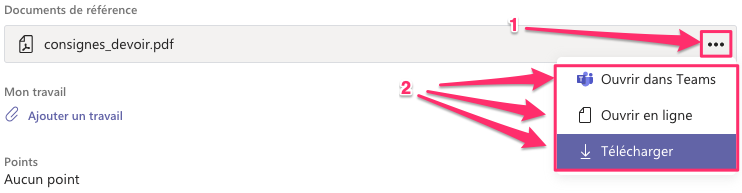
\includegraphics[width=9cm]{./images/teams/choix_pointilles}
\centering
\end{figure}

% REMETTRE SON DEVOIR
\subsection{Remettre son devoir}\label{TeamsRemettreDevoir}

Pour remettre votre devoir, il faut d'abord cliquer sur l'onglet \textit{Ajouter un travail}. 

\begin{figure}[H]
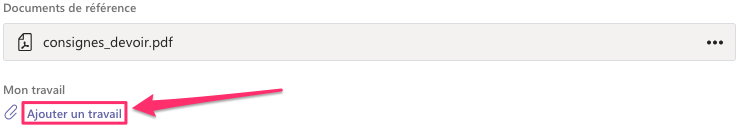
\includegraphics[width=9cm]{./images/teams/ajout}
\centering
\end{figure}

S'ouvre alors une fenêtre qui vous permet de rechercher votre document à partir d'un dossier local relatif à votre ordinateur, à partir du OneDrive ou encore à partir d'une autre équipe.

\begin{figure}[H]
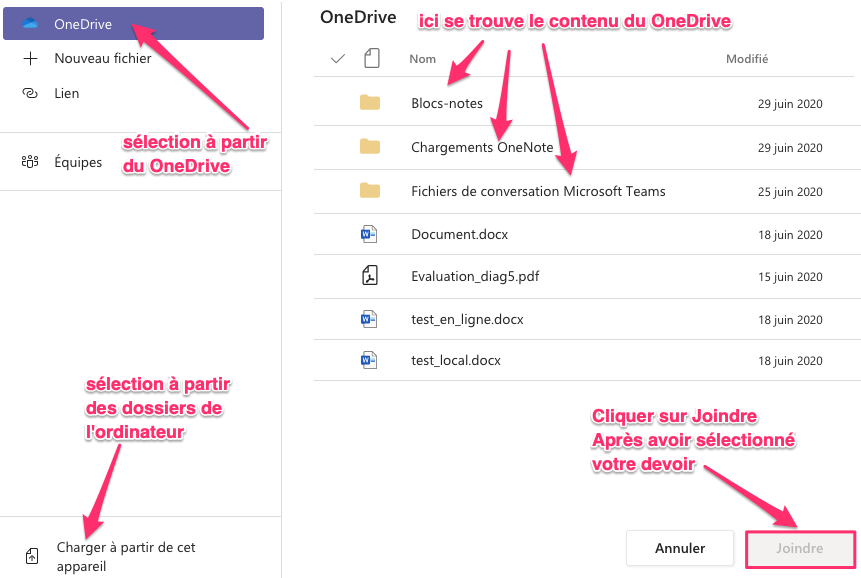
\includegraphics[width=11cm]{./images/teams/selection_devoir}
\centering
\end{figure}

Une fois votre devoir à remettre sélectionné, il suffit de cliquer sur \textit{Joindre}. A ce stade, votre devoir n'est pas encore enregistré. Il faut maintenant choisir \textit{Terminé} pour l'enregistrer.

\begin{figure}[H]
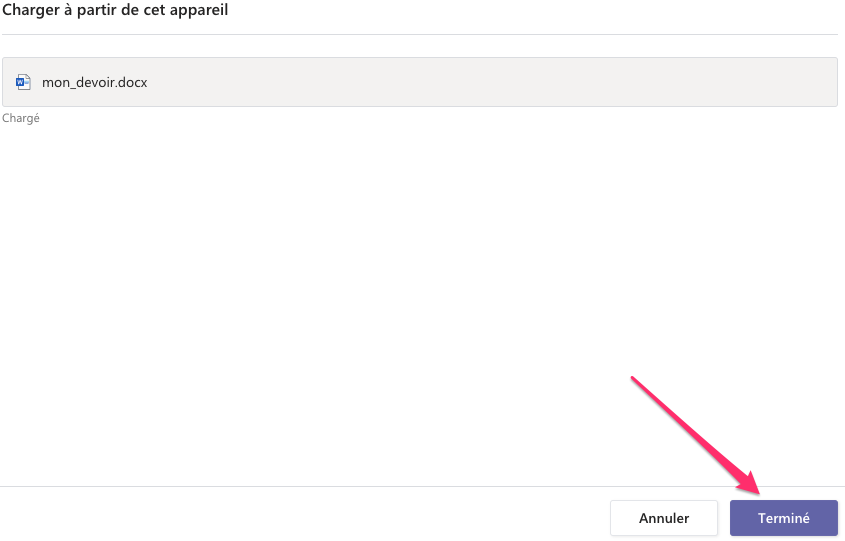
\includegraphics[width=9cm]{./images/teams/ajout2}
\centering
\end{figure}

Vous pouvez également ajouter un autre travail, vous pouvez également télécharger votre devoir afin de vérifier son contenu. Vous pouvez également supprimer votre travail.

\begin{figure}[H]
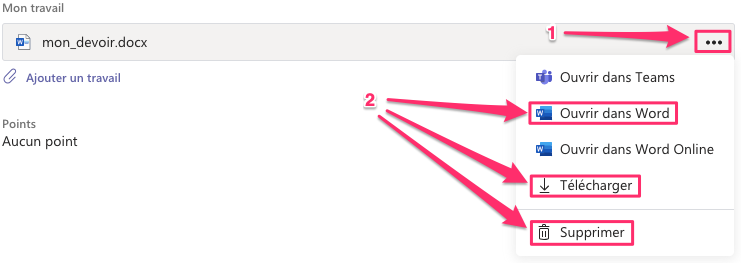
\includegraphics[width=9cm]{./images/teams/ajout3}
\centering
\end{figure}

Attention, votre devoir n'est pas encore remis. il faut maintenant choisir l'onglet \textit{Remettre} pour valider l'envoi de votre devoir. 

\begin{figure}[H]
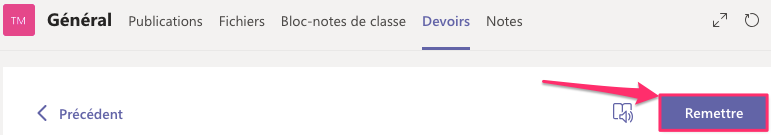
\includegraphics[width=9cm]{./images/teams/ajout4}
\centering
\end{figure}


% ACCEDER A MON CARNET
\section{Accéder à mon bloc-note}

Certains de vos enseignants mettront à votre disposition un bloc-note de classe. C'est un outil très pratique qui permet de prendre des notes et de modifier des fichiers mis à votre disposition, directement depuis Teams.\\

Pour accéder au carnet de classe, cliquez sur \textit{Bloc-notes de classe}, en haut de la page de la classe.

\begin{figure}[H]
	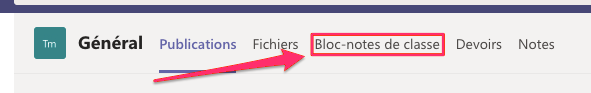
\includegraphics[width=9cm]{./images/teams/acces_bloc_notes_crop}
	\centering
\end{figure}

S'ouvre alors la page d'accueil du bloc-notes. Votre enseignant l'aura probablement adaptée à son cours, elle ne ressemblera donc pas forcément à l'image ci-dessous.

\begin{figure}[H]
	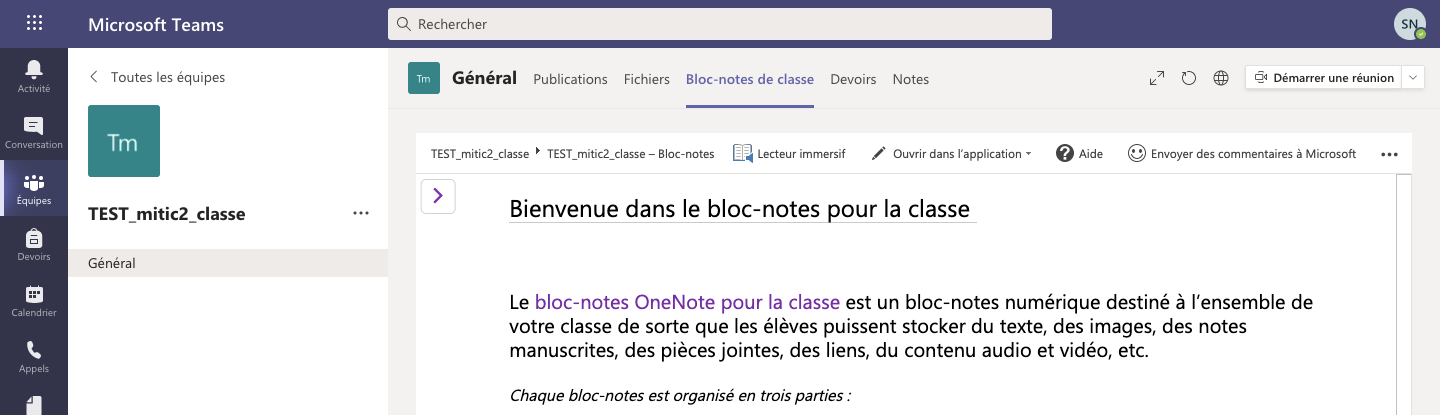
\includegraphics[width=11cm]{./images/teams/ouvrir_menu_bloc_notes_crop}
	\centering
\end{figure}

Cliquez sur la flèche en haut à gauche de l'espace de travail pour ouvrir la liste des bloc-notes. Une section à votre nom apparait, en bas de la liste. Il s'agit d'un espace personnel dans lequel vous pouvez écrire ce que vous voulez, que ce soit pour modifier des fichiers ou prendre des notes. Cliquez sur votre nom pour afficher des sous-sections.

\begin{figure}[H]
	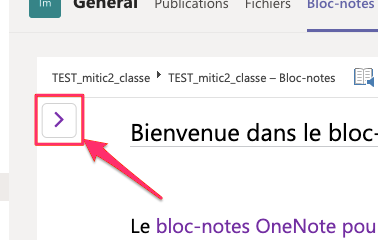
\includegraphics[width=6cm]{./images/teams/ouvrir_liste_dossiers_docs_crop}
	\centering
\end{figure}

Ouvrez la page sans titre, dans la sous-section \textit{Documents}. Ecrivez le titre de votre document. Vous verrez que le titre sera mis à jour dans la liste de documents, à gauche. Si votre liste de sections et documents s'est refermée, il suffit de cliquer sur la flèche, comme tout à l'heure, pour l'afficher à nouveau.\\

Vous pouvez maintenant écrire du texte, ajouter des images, ou modifier ce document comme vous le souhaitez.\\

Si vous souhaitez ajouter une nouvelle page, vous pouvez cliquer sur \textit{+ Page}, en bas. Renommez la nouvelle page en écrivant un titre comme vous venez de le faire.

\begin{figure}[H]
	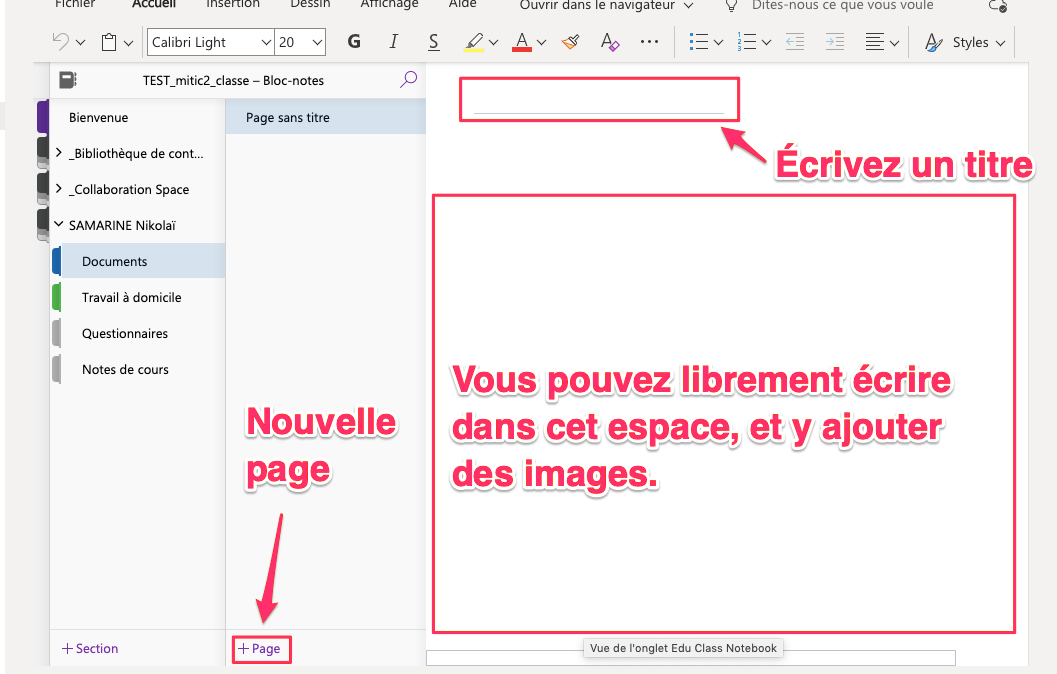
\includegraphics[width=10cm]{./images/teams/sous_section_documents_crop}
	\centering
\end{figure}

En ajoutant et modifiant ainsi des pages, vous allez pouvoir prendre des notes et y accéder via divers appareils, que ce soit depuis la maison ou l'école.

% REJOINDRE UNE VISIO CONFERENCE
\section{Rejoindre une visio-conférence}

Lorsque vous devez assister à un cours à distance, il est nécessaire de rejoindre une visio-conférence déjà commencée. Pour cela, dans l'onglet \textit{Publications}, vous aller trouver une invitation pour participer à une visio-conférence déjà ouverte

\begin{figure}[H]
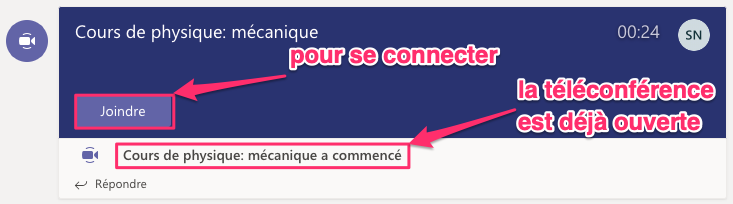
\includegraphics[width=9cm]{./images/teams/video1}
\centering
\end{figure}

Attention, si vous sélectionnez \textit{Demarrer une réunion}, vous allez créer une nouvelle téléconférence et non pas rejoindre la téléconférence déjà programmée pour votre cours.

\begin{figure}[H]
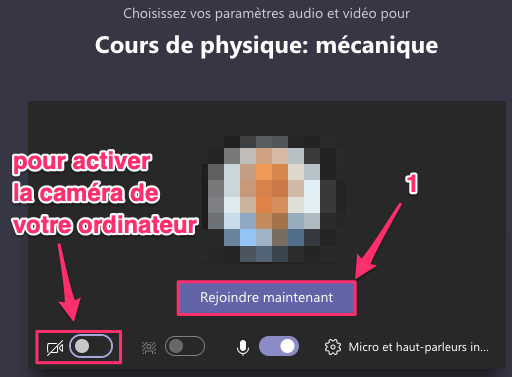
\includegraphics[width=7cm]{./images/teams/video2}
\centering
\end{figure}





% APPARENCE DE LA PAGE D'ACCUEIL
\section{Pour aller plus loin}
\subsection{Apparence de la page d'accueil}

La page d'accueil de Teams se présente sous forme d'une liste d'équipes

\begin{figure}[H]
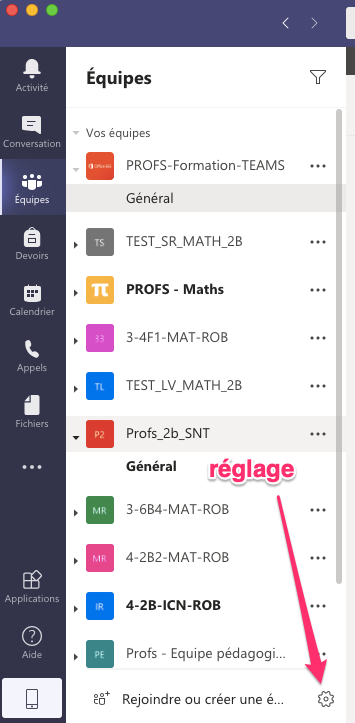
\includegraphics[width=4cm]{./images/teams/accueil_liste}
\centering
\end{figure}

\newpage
ou sous forme d'une grille d'équipes 

\begin{figure}[H]
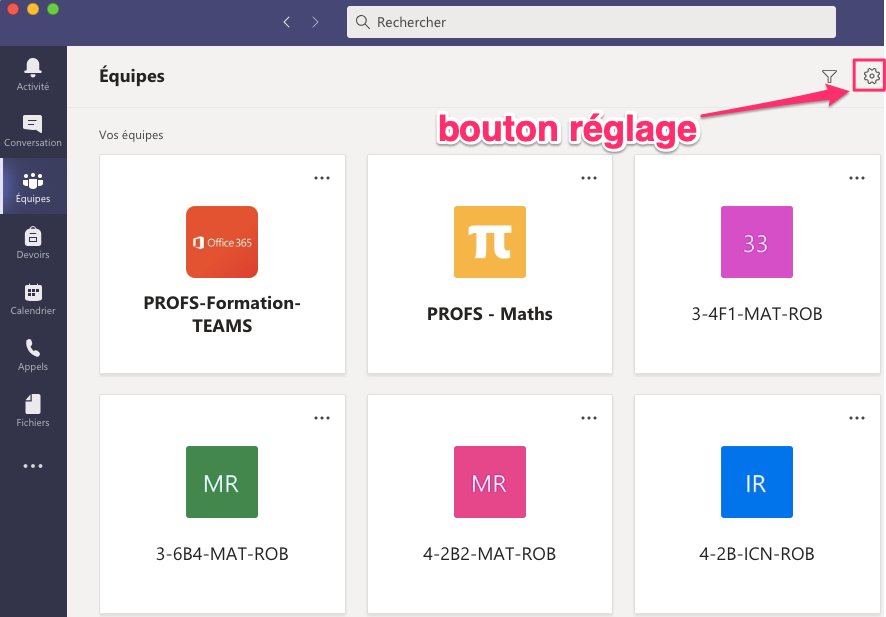
\includegraphics[width=7cm]{./images/teams/accueil_grille}
\centering
\end{figure}

Pour passer d'une forme à l'autre, il faut cliquer sur l'icône 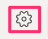
\includegraphics[width=0.8cm]{./images/teams/bouton_parametres}, choisir \textit{Changer d'affichage} dans le menu déroulant, comme dans l'exemple illustré ci-dessous :

\begin{figure}[H]
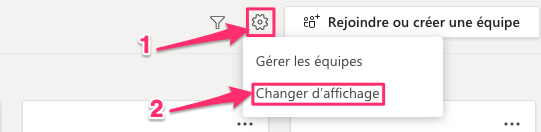
\includegraphics[width=9cm]{./images/teams/changement_liste}
\centering
\end{figure}

Il faut ensuite sélectionner le type d'affichage souhaité entre \textit{Grille} et \textit{Liste}

\begin{figure}[H]
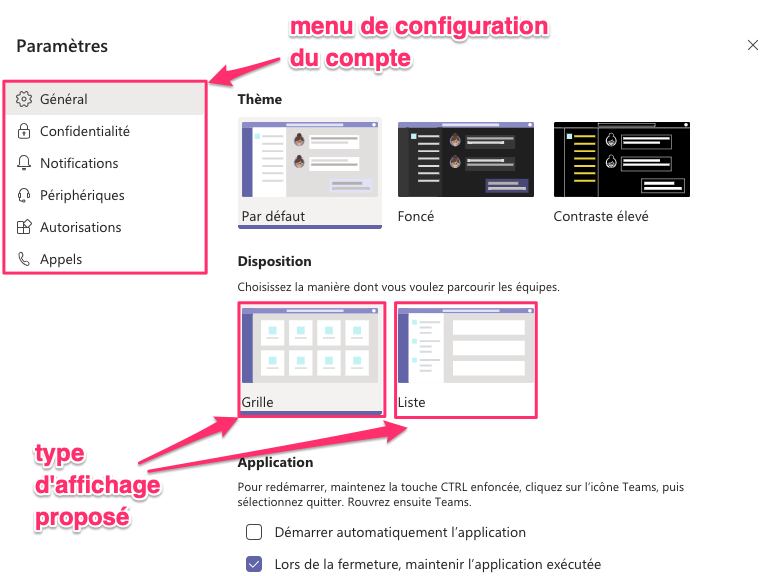
\includegraphics[width=9cm]{./images/teams/choix_parametre}
\centering
\end{figure}

 Pour entrer maintenant dans votre équipe, il suffit de cliquer sur l'icône correspondante

\begin{figure}[H]
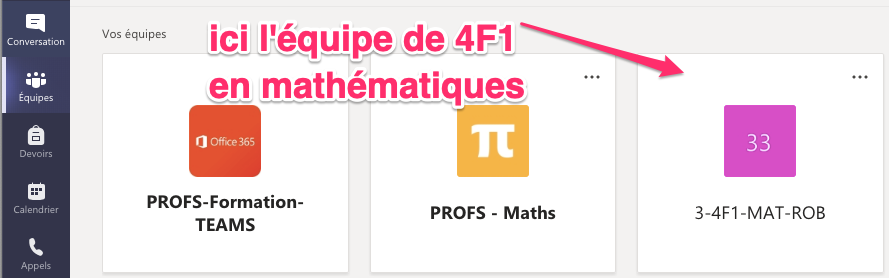
\includegraphics[width=7.5cm]{./images/teams/entree_classe}
\centering
\end{figure}






\section{Séance 1 - utilisation de Geogebra pour construire la droite d'Euler}

construction de médianes, médiatrices, hauteurs, bissectrices, droite d'Euler et cercle d'Euler à partir d'un triangle (Geogebra a déjà été utilisé au cycle) - activité déjà créée\\

matière mathématiques

\section{Séance 2 - découverte Python et module turtle}

découverte de Python par comparaison avec les modules Scratch utilisés au cycle. Utilisation du module Turtle en Python pour créer une répétition de carrés - activité déjà créée\\

matière mathématiques

\section{Séance 22 - découverte Python sur les variables et conditions}

passage de Scratch à Python\\

matière mathématiques

\section{Séance 3  - dessin d'une courbe en Python}

découverte des courbes et surfaces en Python (2D, 3D), changement de couleurs, d'épaisseur de trait, de type de trait. Les codes sources sont donnés aux élèves - activité déjà créée\\

matière mathématiques

\section{Séance 4 - expérience physique et courbes en Python}

 à partir d'une expérience physique, recherche d'informations sur Internet, création d'un fichier csv sur Excel, vérification que le fichier respecte des normes, création d'une courbe Python à partir de ce fichier, ajout de l'unité à un axe et changement de couleur de courbe - activité en cours de création par Nikolai\\

matière sciences physiques

\section{Séaence 5 - résistivité Sebastien Perrad}

à partir de résultats obtenus en physique sur la résistivité, calcul d'un coefficient puis placement des solutions dans un fichier Excel afin de tracer une courbe à partir d'Excel. - activité proposée par Sebastien Perrad, un peu plus difficile que ce que les élèves font au cycle.\\

matière sciences physiques

\section{Séance 6 - de traitement de l'image avec Python}

utilisation des filtres pour tranformer une photo en Python. traitement d'une image en Python, (contraste, luminosité, pixels). Les codes sources sont fournis à l'élève - activité non réalisée\\

 matière dessin ou mathématiques

\section{Séance 7 - calcul littéral - factorisation, développement}

activité 7 : apprendre à factoriser et développer en Python pour vérifier des résultats trouvés manuellement en cours de maths - activité déjà créée et testée en classe. L'activité est assez facile, mais le chapitre sur la factorisation est une bête noire pour les élèves\\

matière mathématiques


\section{Séance 8 - utilisation des moteurs de recherches - social dilemma}

expérience de groupe pour comprendre la réponse fournie par les moteurs de recherche en fonction des recherches antérieures effectuées. Connaissance du mode de rémunération des Gafam et du traitement de l'information. Sensibilisation à l'origine de l'information sur Internet - activité non réalisée.\\

matière Histoire


\section{Séance 9 - statistique descriptive avec Excel}

utilisation de Excel pour les statistiques descriptives (pouvant servir d'appui au programme de maths) - activité non réalisée\\

matière mathématiques

\section{Séance 10 - statistique descriptive avec Python}

utilisation de Python pour les statistiques descriptives (pouvant servir d'appui au programme de maths) - activité non réalisée\\

matière mathématiques

\section{Séance 11 - création site Web avec WordPress}

création d'un site web avec WordPress (prélude à la création d'une page web en Python pour les élèves de seconde bac) - activité non réalisée. site relatif à un événement historique en relation avec le programme d'histoire ou d'économie\\

matière histoire ou économie










\printindex % il faut utiliser en console "makeindex monfichier.idx" pour faire afficher l'index

\end{document}


